% Created 2017-08-31 Thu 13:49
\documentclass[presentation]{beamer}
\usepackage[utf8]{inputenc}
\usepackage[T1]{fontenc}
\usepackage{fixltx2e}
\usepackage{graphicx}
\usepackage{longtable}
\usepackage{float}
\usepackage{wrapfig}
\usepackage{rotating}
\usepackage[normalem]{ulem}
\usepackage{amsmath}
\usepackage{textcomp}
\usepackage{marvosym}
\usepackage{wasysym}
\usepackage{amssymb}
\usepackage{hyperref}
\tolerance=1000
\setbeamertemplate{navigation symbols}{}
\usetheme{default}
\author{Week 2 - PSYC 5316}
\date{September 4, 2017}
\title{Maximum Likelihood Estimation}
\hypersetup{
  pdfkeywords={},
  pdfsubject={},
  pdfcreator={Emacs 25.2.1 (Org mode 8.2.10)}}
\begin{document}

\maketitle

\begin{frame}[label=sec-1]{Recall}
Last time, we gave a formal definition for a \alert{probability function}.  An example was the \emph{binomial} distribution for $N$ independent Bernoulli trials (e.g., coin flips):

\[
f(x\mid \theta) = {N\choose x} \theta^x(1-\theta)^{N-x}
\]

where $x$ = \# of successes, and $\theta$ = probability of success.
\end{frame}

\begin{frame}[fragile,label=sec-2]{Probability function}
 Suppose $N=20$ and $\theta=0.7$.  

\begin{verbatim}
barplot(dbinom(0:20,size=20,prob=0.7),
        names.arg=0:20,
        ylab="p(x)",
        xlab="x")
\end{verbatim}

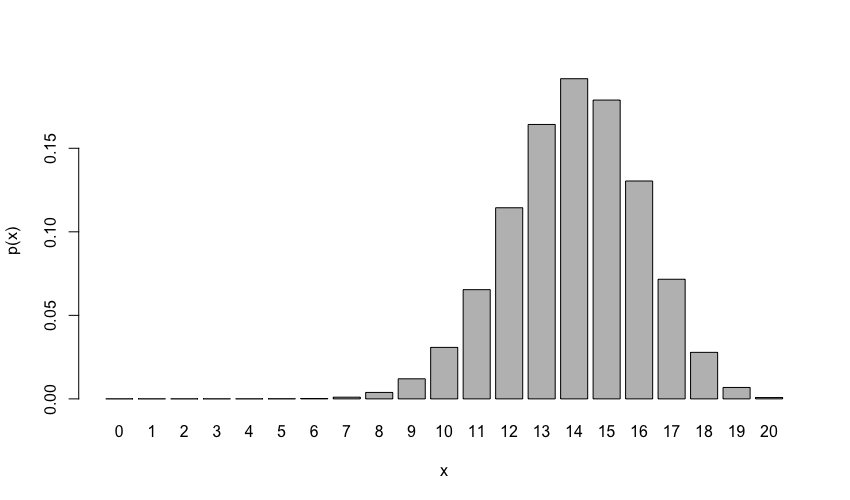
\includegraphics[width=.9\linewidth]{figures/week2/binom.png}
\end{frame}

\begin{frame}[label=sec-3]{Data and parameters}
\[
f(x\mid \theta) = {N\choose x} \theta^x(1-\theta)^{N-x}
\]

\vspace{1cm}

This function gives us the probability of \alert{data}, \emph{given} a specific \alert{parameter}
\end{frame}

\begin{frame}[label=sec-4]{Data and parameters}
What if we switched these?

\[
f(\theta \mid x) = {N\choose x} \theta^x(1-\theta)^{N-x}
\]

\vspace{1cm}

This function then gives us the likelihood of a range of \alert{parameters}, \emph{given} a specific \alert{data point}
\end{frame}

\begin{frame}[fragile,label=sec-5]{Likelihood function}
 Suppose we observed 12 successes in 20 trials:

\begin{verbatim}
theta=seq(from=0, to=1, by=0.01)
plot(theta, dbinom(x=12, size=20, prob=theta), 
     type="l",ylab="likelihood")
\end{verbatim}

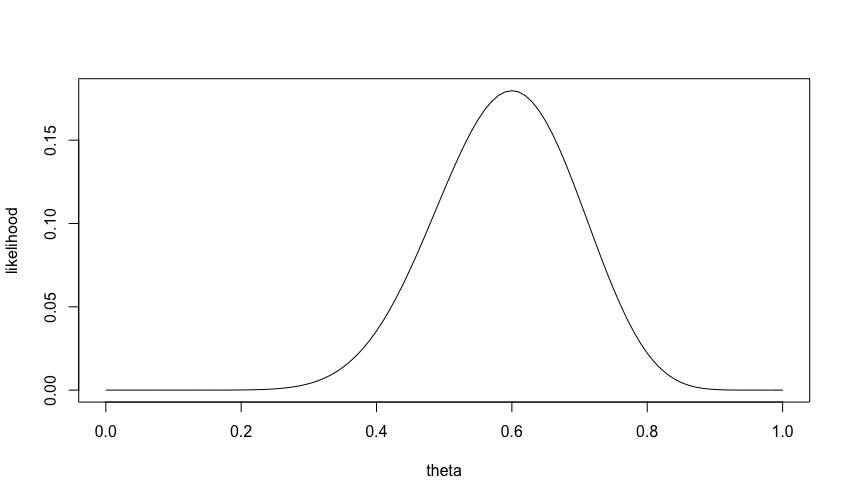
\includegraphics[width=.9\linewidth]{figures/week2/likelihood.png}
\end{frame}

\begin{frame}[label=sec-6]{Likelihood function}
Suppose we observed 12 successes in 20 trials:

\vspace{1cm}

Natural question -- what value of $\theta$ is \alert{most likely}, given the data?

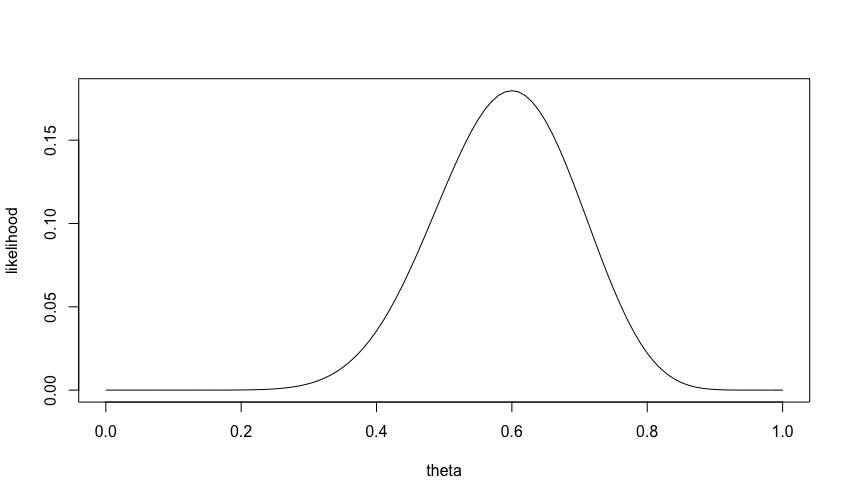
\includegraphics[width=.9\linewidth]{figures/week2/likelihood.png}
\end{frame}

\begin{frame}[label=sec-7]{Likelihood function}
Suppose we observed 12 successes in 20 trials:

\vspace{1cm}

Natural question -- what value of $\theta$ is \alert{most likely}, given the data?

Answer: $\theta=0.6$

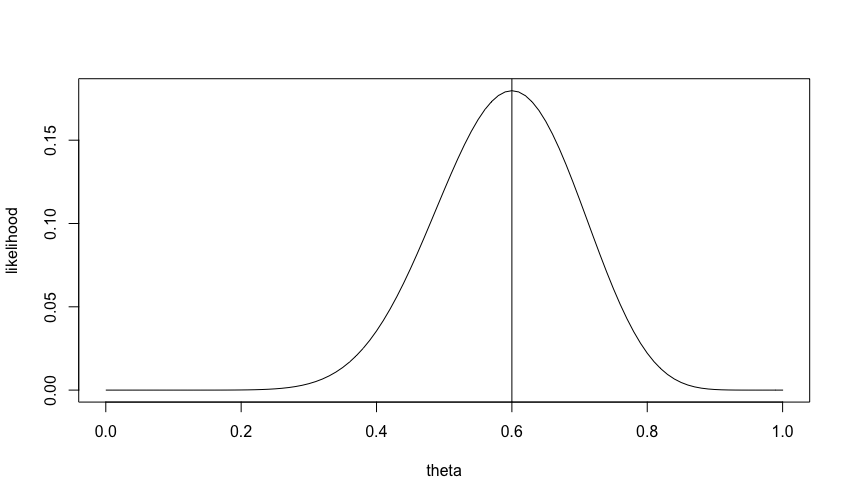
\includegraphics[width=.9\linewidth]{figures/week2/maxLikelihood.png}
\end{frame}

\begin{frame}[label=sec-8]{Maximum likelihood estimation}
A key problem in statistical inference is how to infer from \alert{sample data} to \alert{population parameters}.

\vspace{1cm}

Maximum likelihood estimation is one solution to this problem
\end{frame}

\begin{frame}[label=sec-9]{Maximum likelihood estimation}

\includegraphics[width=.9\linewidth]{figures/week2/mlePaper.png}
\end{frame}

\begin{frame}[label=sec-10]{Maximum likelihood estimation}
Basic workflow:
\begin{enumerate}
\item collect data
\item decide on a "model" for the data (e.g., binomial, normal, etc.)
\item define a likelihood function based on the underlying model
\item find the parameter value(s) that \alert{maximize} the likelihood function
\end{enumerate}
\end{frame}


\begin{frame}[label=sec-11]{Three examples}
We will do three examples of MLE:
\begin{enumerate}
\item binomial model
\item normal model
\item ex-Gaussian model
\end{enumerate}
\end{frame}


\begin{frame}[label=sec-12]{Example 1}
Suppose that in a sequence of 20 coin flips, we observe 12 successes ("heads").  What is the maximum likelihood estimate for $\theta$?

\vspace{5mm}

Step 1 -- collect data
\begin{itemize}
\item done: we observed $x=12$ successes
\end{itemize}
\end{frame}

\begin{frame}[label=sec-13]{Example 1}
Suppose that in a sequence of 20 coin flips, we observe 12 successes ("heads").  What is the maximum likelihood estimate for $\theta$?

\vspace{5mm}

Step 2 -- choose a model
\begin{itemize}
\item assume a binomial model
\end{itemize}

\[
x \sim \text{Binomial}(\theta, n=20)
\]
\end{frame}

\begin{frame}[fragile,label=sec-14]{Example 1}
 Suppose that in a sequence of 20 coin flips, we observe 12 successes ("heads").  What is the maximum likelihood estimate for $\theta$?

\vspace{5mm}

Step 3 -- define likelihood function
\begin{itemize}
\item Note: we will actually define the "negative log-likelihood" function
\end{itemize}

\begin{verbatim}
nll.binom <- function(data,par){
  return(-log(dbinom(data, size = 20, prob = par)))
}
\end{verbatim}
\end{frame}


\begin{frame}[fragile,label=sec-15]{Example 1}
 Suppose that in a sequence of 20 coin flips, we observe 12 successes ("heads").  What is the maximum likelihood estimate for $\theta$?

\vspace{5mm}

Step 4 -- find parameter that maximizes the likelihood function
\begin{itemize}
\item Note: we will actually \alert{minimize} the negative log-likelihood
\end{itemize}

\begin{verbatim}
optim(par=0.5, fn=nll.binom, data=12)
\end{verbatim}
\end{frame}


\begin{frame}[label=sec-16]{Example 1}
Suppose that in a sequence of 20 coin flips, we observe 12 successes ("heads").  What is the maximum likelihood estimate for $\theta$?

\vspace{5mm}

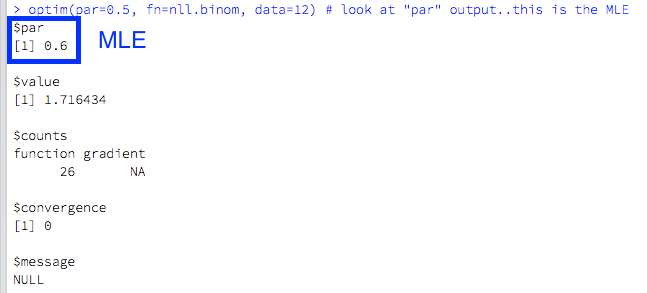
\includegraphics[width=.9\linewidth]{figures/week2/binomOutput.png}
\end{frame}


\begin{frame}[fragile,label=sec-17]{Example 2}
 The following command will load a data set into R, consisting of 1000 observations.  Fit the data with a normal model and find MLEs for mean and standard deviation.

\vspace{5mm}

Step 1: collect data

\begin{verbatim}
data <- read.csv("https://git.io/v58i8")
\end{verbatim}
\end{frame}


\begin{frame}[fragile,label=sec-18]{Example 2}
 The following command will load a data set into R, consisting of 1000 observations.  Fit the data with a normal model and find MLEs for mean and standard deviation.

\vspace{5mm}

Step 1.5: before choosing a model, look at the distribution

\begin{verbatim}
hist(data$x)
\end{verbatim}

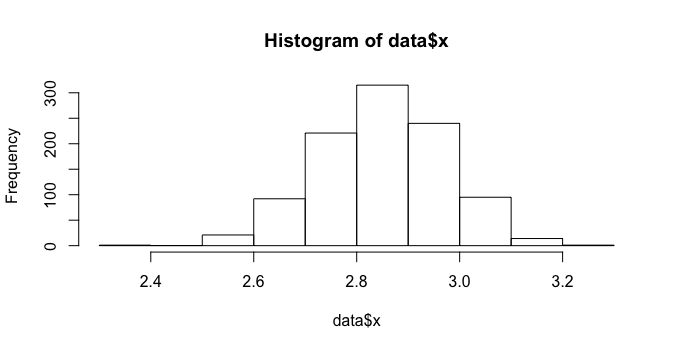
\includegraphics[width=.9\linewidth]{figures/week2/normalHistogram.png}
\end{frame}


\begin{frame}[fragile,label=sec-19]{Example 2}
 The following command will load a data set into R, consisting of 1000 observations.  Fit the data with a normal model and find MLEs for mean and standard deviation.

\vspace{5mm}

Step 1.5: before choosing a model, look at the distribution

\begin{verbatim}
plot(density(data$x))
\end{verbatim}

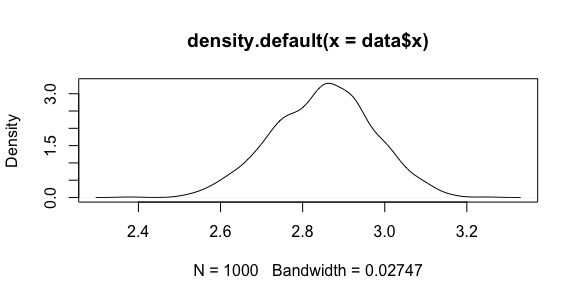
\includegraphics[width=.9\linewidth]{figures/week2/normalDensity.png}
\end{frame}


\begin{frame}[label=sec-20]{Example 2}
The following command will load a data set into R, consisting of 1000 observations.  Fit the data with a normal model and find MLEs for mean and standard deviation.

\vspace{5mm}

Step 2: choose a model
\begin{itemize}
\item assume a normal model
\end{itemize}

\[
x \sim \text{Normal}(\mu,\sigma)
\]
\end{frame}


\begin{frame}[fragile,label=sec-21]{Example 2}
 The following command will load a data set into R, consisting of 1000 observations.  Fit the data with a normal model and find MLEs for mean and standard deviation.

\vspace{5mm}

Step 3: define likelihood function

\begin{verbatim}
nll.normal <- function(data,par){
  return(-sum(log(dnorm(data, mean=par[1], sd=par[2]))))
}
\end{verbatim}
\end{frame}


\begin{frame}[fragile,label=sec-22]{Example 2}
 The following command will load a data set into R, consisting of 1000 observations.  Fit the data with a normal model and find MLEs for mean and standard deviation.

\vspace{5mm}

Step 4: find parameters that maximize the likelihood function

\begin{verbatim}
optim(par=c(1,0.1), fn=nll.normal, data=data$x)
\end{verbatim}
\end{frame}


\begin{frame}[label=sec-23]{Example 2}
The following command will load a data set into R, consisting of 1000 observations.  Fit the data with a normal model and find MLEs for mean and standard deviation.

\vspace{5mm}

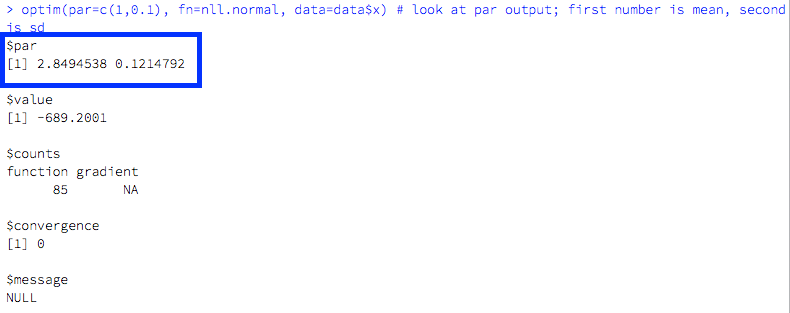
\includegraphics[width=.9\linewidth]{figures/week2/normalOutput.png}
\end{frame}

\begin{frame}[fragile,label=sec-24]{Example 2}
 As a check, we can see how well our model "fits" the data:

\begin{verbatim}
x=seq(-3,4,0.01)
plot(density(data$x))
lines(x,dnorm(x,mean=2.85, sd=0.12),lty=2)
\end{verbatim}

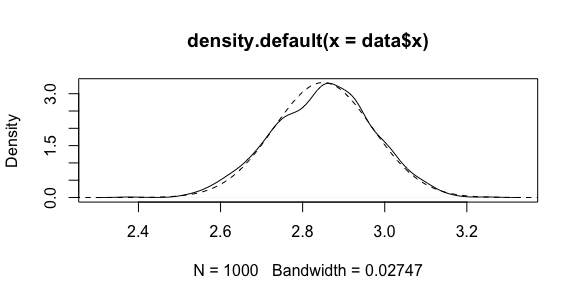
\includegraphics[width=.9\linewidth]{figures/week2/normalFit.png}
\end{frame}

\begin{frame}[fragile,label=sec-25]{Example 3}
 Step 1: collect data

\vspace{5mm}

Here is a data set of 1000 response times (RTs) in a mental arithmetic task, followed by a plot of the data.  

\begin{verbatim}
data <- read.csv("https://git.io/v58yI")
plot(density(data$rt))
\end{verbatim}

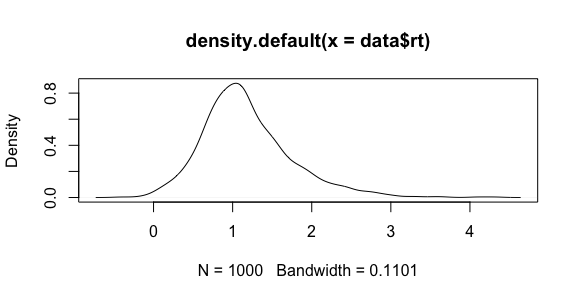
\includegraphics[width=.9\linewidth]{figures/week2/rtPlot.png}
\end{frame}



\begin{frame}[label=sec-26]{Example 3}
Step 2: choose a model
\begin{itemize}
\item distributions with long rightward tails can be modeled by an ex-Gaussian distribution, which is essentially a combination of the Gaussian (normal) distribution with an exponential distribution
\end{itemize}

\vspace{3mm}

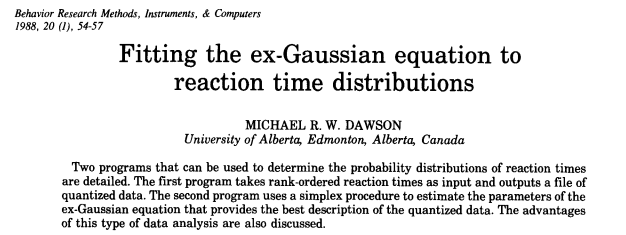
\includegraphics[width=.9\linewidth]{figures/week2/exGpaper.png}
\end{frame}

\begin{frame}[label=sec-27]{Example 3}
Step 2: choose a model
\begin{itemize}
\item distributions with long rightward tails can be modeled by an ex-Gaussian distribution, which is essentially a combination of the Gaussian (normal) distribution with an exponential distribution
\end{itemize}

\[
rt \sim \text{exGaussian}(\mu, \sigma, \tau)
\]

\begin{itemize}
\item $\mu$ = mean of normal component
\item $\sigma$ = sd of normal component
\item $\tau$ = rate of exponential component
\end{itemize}
\end{frame}

\begin{frame}[fragile,label=sec-28]{Example 3}
 Step 3: define likelihood function
\begin{itemize}
\item ExGaussian is not already a function in R.  So, we'll build it ourselves.
\item note: just copy from the week2.R script!
\end{itemize}

\begin{verbatim}
dexg <- function(x, mu, sigma, tau){
  return((1/tau)*exp((sigma^2/(2*tau^2)) -
  (x-mu)/tau)*pnorm((x-mu)/sigma-(sigma/tau)))
}
\end{verbatim}
\end{frame}


\begin{frame}[fragile,label=sec-29]{Example 3}
 Step 3: define likelihood function

\begin{verbatim}
nll.exg <- function(data,par){
  return(-sum(log(dexg(data, 
  mu=par[1], 
  sigma=par[2], 
  tau=par[3]))))
}
\end{verbatim}
\end{frame}


\begin{frame}[fragile,label=sec-30]{Example 3}
 Step 4: find parameters that maximize likelihood function

\begin{verbatim}
optim(par=c(0,0.1,0.1), fn=nll.exg, data = data$rt)
\end{verbatim}

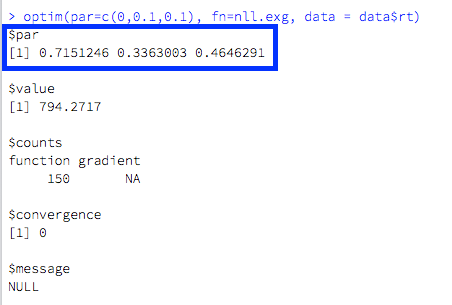
\includegraphics[width=.9\linewidth]{figures/week2/exGoutput.png}
\end{frame}


\begin{frame}[fragile,label=sec-31]{Example 3}
 As before, let's check our model fit

\begin{verbatim}
x=seq(0,4,0.1)
plot(density(data$rt))
lines(x,dexg(x,mu=0.715, sigma=0.336, tau=0.465),lty=2)
\end{verbatim}

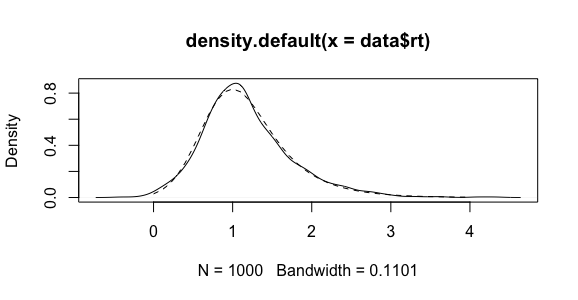
\includegraphics[width=.9\linewidth]{figures/week2/exGfit.png}
\end{frame}
% Emacs 25.2.1 (Org mode 8.2.10)
\end{document}